\chapter{Mise en oeuvre de la solution}

\label{sec:realisation}

\begin{fquote}
Dans ce chapitre, on va présenter les outils utilisés pour la mise en oeuvre de la solution PIM ainsi qu’un aperçu des différentes vues et interfaces de cette solution.
\end{fquote}

\clearpage

\section{Introduction :}

Une des étapes de la vie d’un projet, aussi importante que la conception, est l’implémentation.

\medskip

Cette étape constitue la phase d’achèvement et d’aboutissement du projet. Pour accomplir cette tâche avec succès il faut savoir utiliser les outils adéquats et nécessaires. Ce choix d’outils peut influencer la qualité du produit obtenu et donc nécessite une attention particulière et doit se baser sur les besoins du projet et le résultat escomptés.

\medskip

Ce chapitre présente l’environnement technique du travail ainsi que le choix pris en matière d’environnement logiciel. 

\section{Outils et technologies utilisées :}
\subsection{La plateforme Java EE}

Java EE ou Java Enterprise Edition (récemment renommée Jakarta EE) est une norme proposée par la société Oracle, portée par un consortium de sociétés internationales, visant à définir un standard de développement d’applications d’entreprises multi-niveaux\cite{wiki:java}.

\medskip

Cette plate-forme est fortement orientée serveur et dédiée au développement et à l’exécution d’applications distribuées. Elle permet la simplification du processus de développement. En effet, JEE simplifie le contrôle et la gestion des ressources système en fournissant des méthodes permettant de gérer les transactions et la mise en commun des ressources.


\subsection{La plateforme SAP Hybris}

Hybris est une solution e-commerce créée en Allemagne, en 1997. Dès le début, la solution a ciblé son développement sur le « \textit{e-commerce} », le « \textit{PIM étendu} » et le « \textit{multi canal} »\cite{wiki:hybris}.


\medskip

Alors que certaines solutions sont clairement bâties pour faire la partie Front (produire du HTML pour faire des sites web), Hybris pense que le coeur du sujet, c’est pas le front, c’est le catalogue. L’idée, est de se dire qu’entre l’ERP, le système d’information de l’entreprise, et les sites Front, il y a besoin d’un middleware\cite{wiki:hybris}.
\medskip

Ce référentiel sera souvent alimenté par un système de plus bas niveau (ERP ou équivalent). A partir de ce référentiel, l’autre axe clé de Hybris, c’est le multi canal. En effet, Hybris permet de publier de manière cohérente, vers les différents canaux de vente : Web, mobile, magasin, etc…
\medskip

La platforme SAP Hybris repose sur des standards ouverts, qui conjugue l’efficacité et l’extensibilité afin d’offrir des capacités infinies d’innovation et de devenir la plate-forme de commerce la plus performante du marché. Ainsi la platforme repose sur plusieurs outils et frameworks open source et standardisés parmi lesquels on trouve :

\begin{itemize}
\medskip
    \item[$\bullet$] \textbf{Le Framework Spring\footnote{\url{https://spring.io/}} :} Un framework libre fournit un modèle complet de programmation et de configuration pour les applications d’entreprise modernes basées sur JEE. Le framework s'appuie principalement sur les principes de l'IOC (Inversion of Control) et de MVC (Model View Controller) \cite{wiki:spring}.
    \medskip

    \item[$\bullet$] \textbf{Apache Tomcat\footnote{\url{http://tomcat.apache.org/}} :} C'est un conteneur web libre de servlets et JSP Java EE. Issu du projet Jakarta. Il incorpore également un serveur HTTP\cite{wiki:tomcat}.
    
    % , c’est un des nombreux projets de l’Apache Software Foundation. Il implémente les spécifications des servlets et des JSP du Java Community Process, et paramétrable par des fichiers XML et des propriétés, et inclut des outils pour la configuration et la gestion.
    \medskip

    \item[$\bullet$] \textbf{Apache Solr\footnote{\url{https://lucene.apache.org/solr/}} :} C'est le moteur de recherche et d’indexation de référence dans le monde du libre. Basé sur la librairie Lucene, il dispose de nombreuses fonctionnalités avancées comme la recherche par facettes, la suggestion orthographique et la recherche par similarité \cite{wiki:solr}.
    \medskip

    \item[$\bullet$] \textbf{ZK Framework\footnote{\url{https://www.zkoss.org/}} :} C'est un framework open source web 2.0, proposant une interaction utilisateur riche. ZK permet tout autant de définir rapidement des interfaces graphiques via une syntaxe XML ou un éditeur Wysiwyg qui permet de manipuler directement les objets en Java \cite{wiki:zk}.
    \medskip
    
    \item[$\bullet$] \textbf{Apache Ant\footnote{\url{https://ant.apache.org/}} :} Ant est un logiciel créé par la fondation Apache qui vise à automatiser les opérations répétitives du développement de logiciel telles que la compilation, la génération de documents ou l'archivage au format JAR, à l'instar des logiciels Make. Ant est écrit en Java et son nom est un acronyme pour « Another Neat Tool » \cite{wiki:ant}.
    

\end{itemize}

\medskip

La plateforme SAP Hybris dispose par défaut des espaces d'administration suivants :

\begin{itemize}
\medskip
    \item[$\bullet$] \textbf{Le Framework Backoffice :} C'est la nouvelle version de l'encien HMC (Hybris Management Console), une interface backend du système qui permet de gérer les utilisateurs, les marchés et leurs catalogues de produits et les différents types du systèmes, il permet les opérations de création, mise à jour, suppression et de recherche à travers des millions d’articles\cite{sap}.
    \medskip
    \item[$\bullet$] \textbf{HAC (Hybris Administration Console) :} C’est une interface backend du système, il permet d’effectuer des opérations d’administrations comme la supervision des performances système, la modification à chaud des paramètres généraux, l’administration du cache système, de session, d’accès au logs etc\cite{sap}.
\end{itemize}

\subsection{Outils de développement et de collaboration :}

\subsubsection{L'IDE IntelliJ IDEA :} Également appelé « IntelliJ », « IDEA » ou « IDJ » est un environnement de développement intégré de technologie Java destiné au développement de logiciels informatique. Il est développé par JetBrains\footnote{\url{https://www.jetbrains.com/idea/}} (anciennement « IntelliJ ») et disponible en deux versions, l'une communautaire, open source, sous licence Apache 2 et l'autre propriétaire, protégée par une licence commerciale \cite{wiki:intellij}.

\subsubsection{Le système de contrôle des versions GIT :} C'est un logiciel libre de gestion de versions, créé par Linus Torvalds(le créateur du noyau Linux), c’est un outil bas niveau, qui se veut simple et très performant, dont la principale tâche est de gérer l’évolution du contenu d’une arborescence. Il fonctionne en mode distribué avec un serveur distant\cite{wiki:git}.

\subsubsection{Atlassian JIRA :} C'est un système de suivi de bugs, un système de gestion des incidents, et un système de gestion de projets développé par Atlassian. Jira\footnote{\url{https://www.atlassian.com/software/jira}} n'est pas un acronyme mais une troncation par aphérèse de Gojira\cite{wiki:jira}.

\section{Quelques interfaces de la plate-forme}
Les différentes interfaces qu'on présentera par la suite sont basé sur des composants ou bien des widgets d'Hybris qu'ils ont été personnalisé et évolués selon le besoin de la plate-forme.

\subsection{La page de Login}
La figure \ref{fig:login}  représente la page de login des utilisateurs. Cette page est composée des éléments suivants:
\medskip
\begin{enumerate}
    \item Logo
    \smallskip
    \item Formulaire d'authentification
    \smallskip
    \item Liste des langues disponibles
\end{enumerate}
\medskip

\begin{figure}[ht]
  \centering
  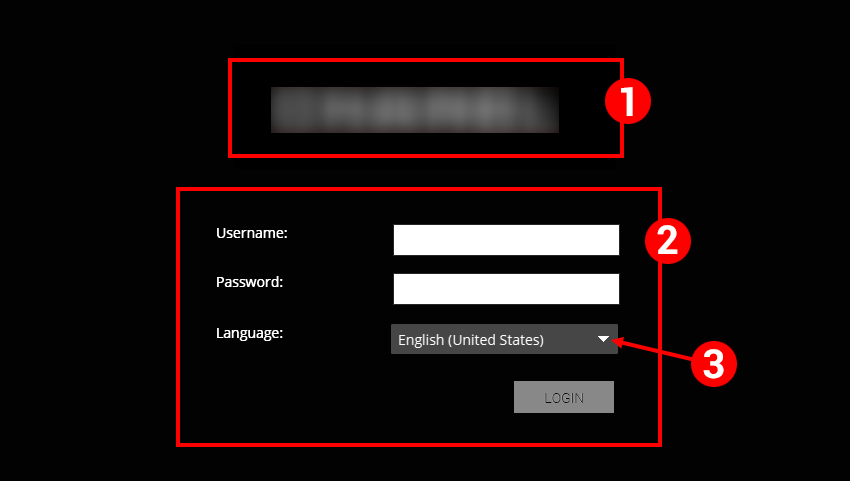
\includegraphics[width=16cm]{login-page.png}
  \caption{La page du login de la platforme PIM.}
  \label{fig:login}
\end{figure}
\FloatBarrier


\subsection{La Vue Administration}

La vue Administration regroupe toutes les opérations de gestion des entités du PIM qu'elle soient natives à hybris comme les cronjob, les employés, les catalogues etc... ou celles spécifiquement crées pour le projet.
\bigskip

Cette vue est présentée dans les deux figures \ref{fig:admin} \ref{fig:admin-category} est composé des éléments suivants :

\begin{enumerate}
    \item Le menu d'administration qui regroupe les élément administrable dans le site sous forme d'arbres.
    \medskip
    \item Le composant de recherche dans les éléments/types du menu d'administration.
    \medskip
    \item Le composant de recherche dans la liste des objets de l'élément/type sélectionné.
    \medskip
    \item La liste des objets disponibles pour l'élément/le type sélectionné.
    \medskip
    \item Le composant d'édition des informations de l'objet sélectionne dans la liste 4.
    \medskip
    \item Les icônes de déconnexion, langues, profiles et d'autres natives a Hybris. 
\end{enumerate}

Dans la figure \ref{fig:admin} le type \textbf{Réference} est sélectionné alors que dans la figure \ref{fig:admin-category} le type de catégorie \textbf{Communication Fonctionnality} est sélectionnée: 


\begin{figure}[ht]
  \centering
  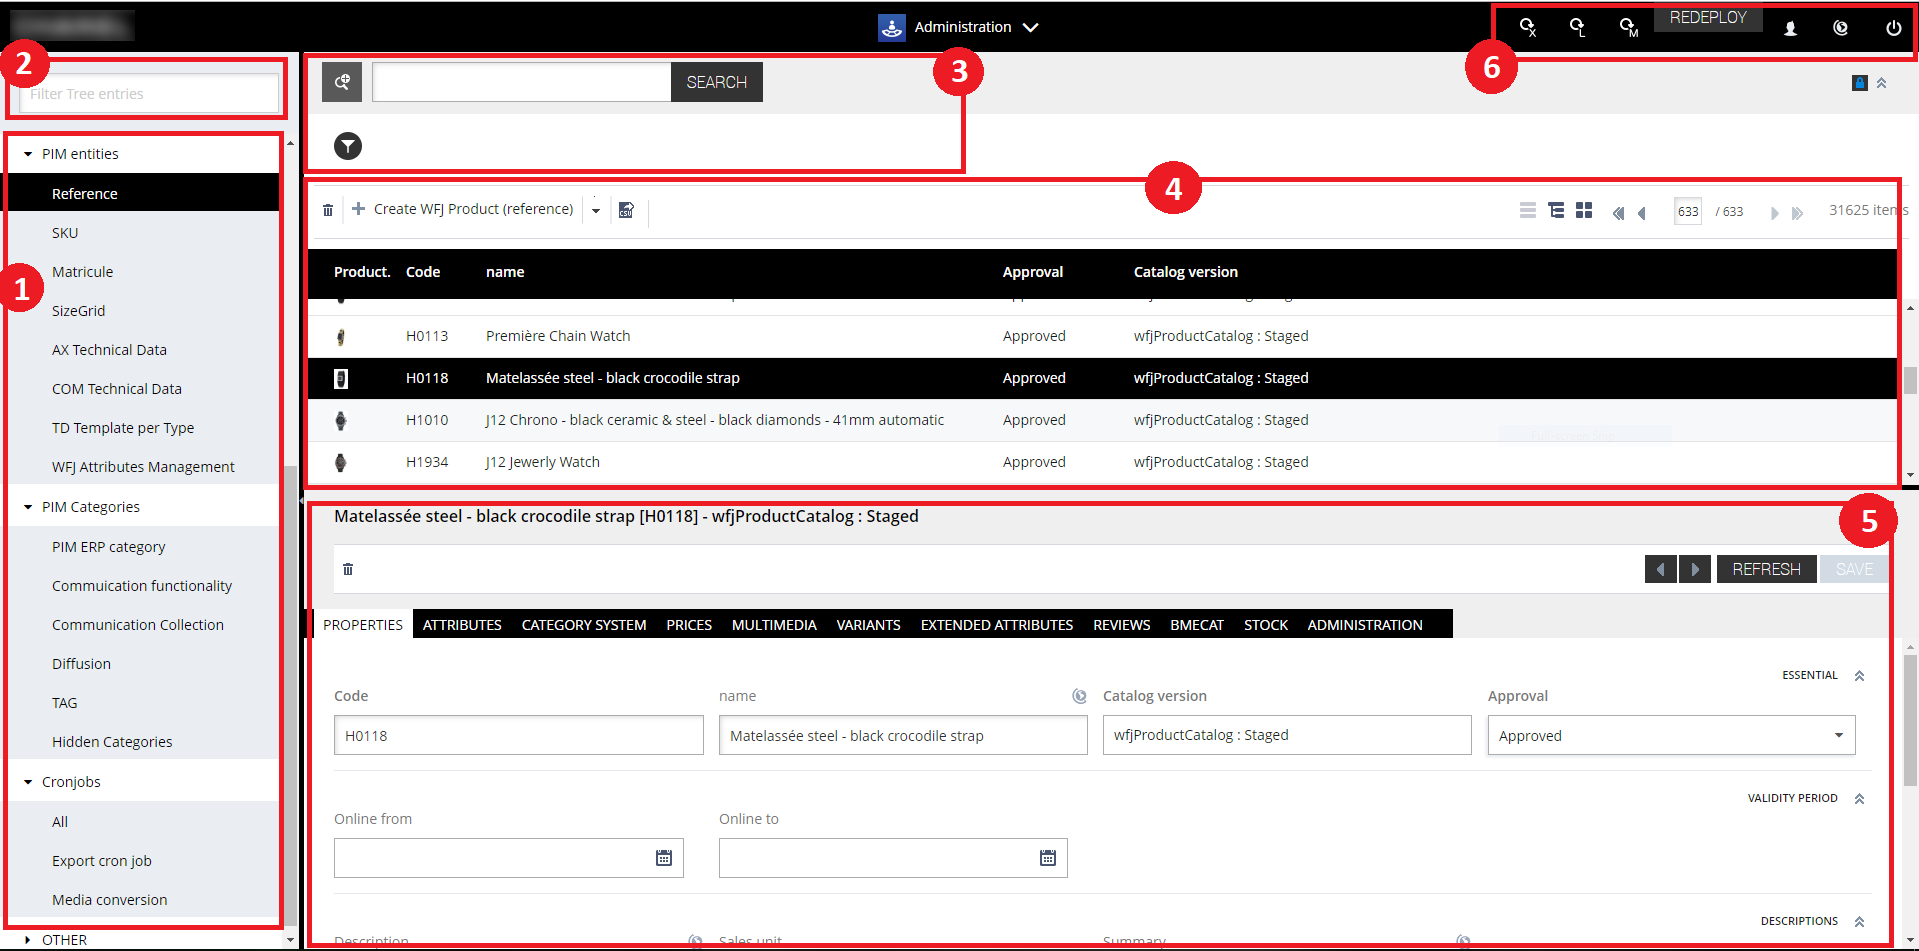
\includegraphics[width=16cm]{admin.PNG}
  \caption{La vue Administration de la plate-forme PIM.}
  \label{fig:admin}
\end{figure}
\FloatBarrier

\begin{figure}[ht]
  \centering
  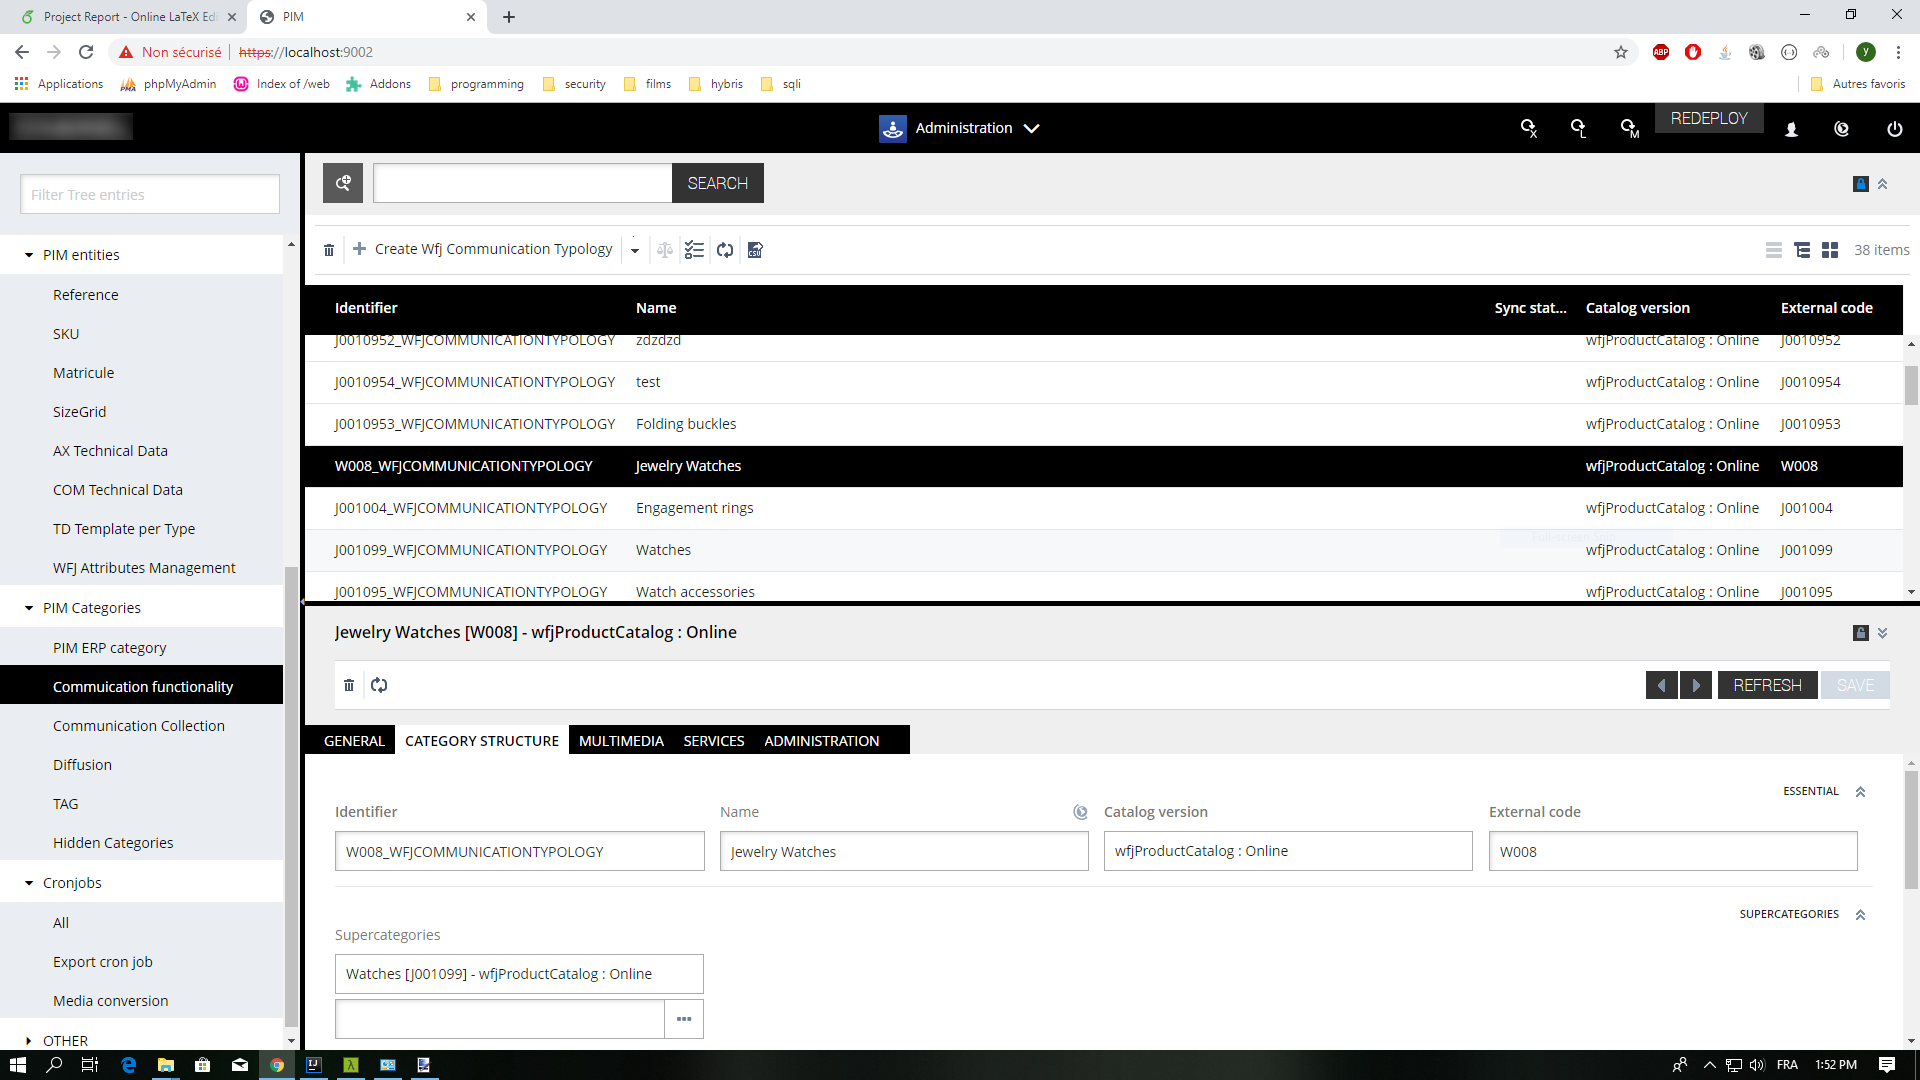
\includegraphics[width=16cm]{admin_category.PNG}
  \caption{La vue Administration avec un type de catégories sélectionnée.}
  \label{fig:admin-category}
\end{figure}
\FloatBarrier

\subsection{La Vue Catalogue}

La vue catalogue présenté dans la figure \ref{fig:ctalog} est une espace de gestion avancé des produits du catalogue, elle est principalement composée des éléments suivants :

\begin{enumerate}
    \item Les composants de filtrage selon les catégories et les filtres prédéfinis.
    \item Le composant de recherche des produits.
    \item La liste des produits recherchés.
    \item Le nom de la vue "Wfj Catalog".
    \item L'image et la présentation du produit sélectionné.
    \item Le composant d'édition avancé des information du produit sélectionné.
\end{enumerate}

\begin{figure}[ht]
  \centering
  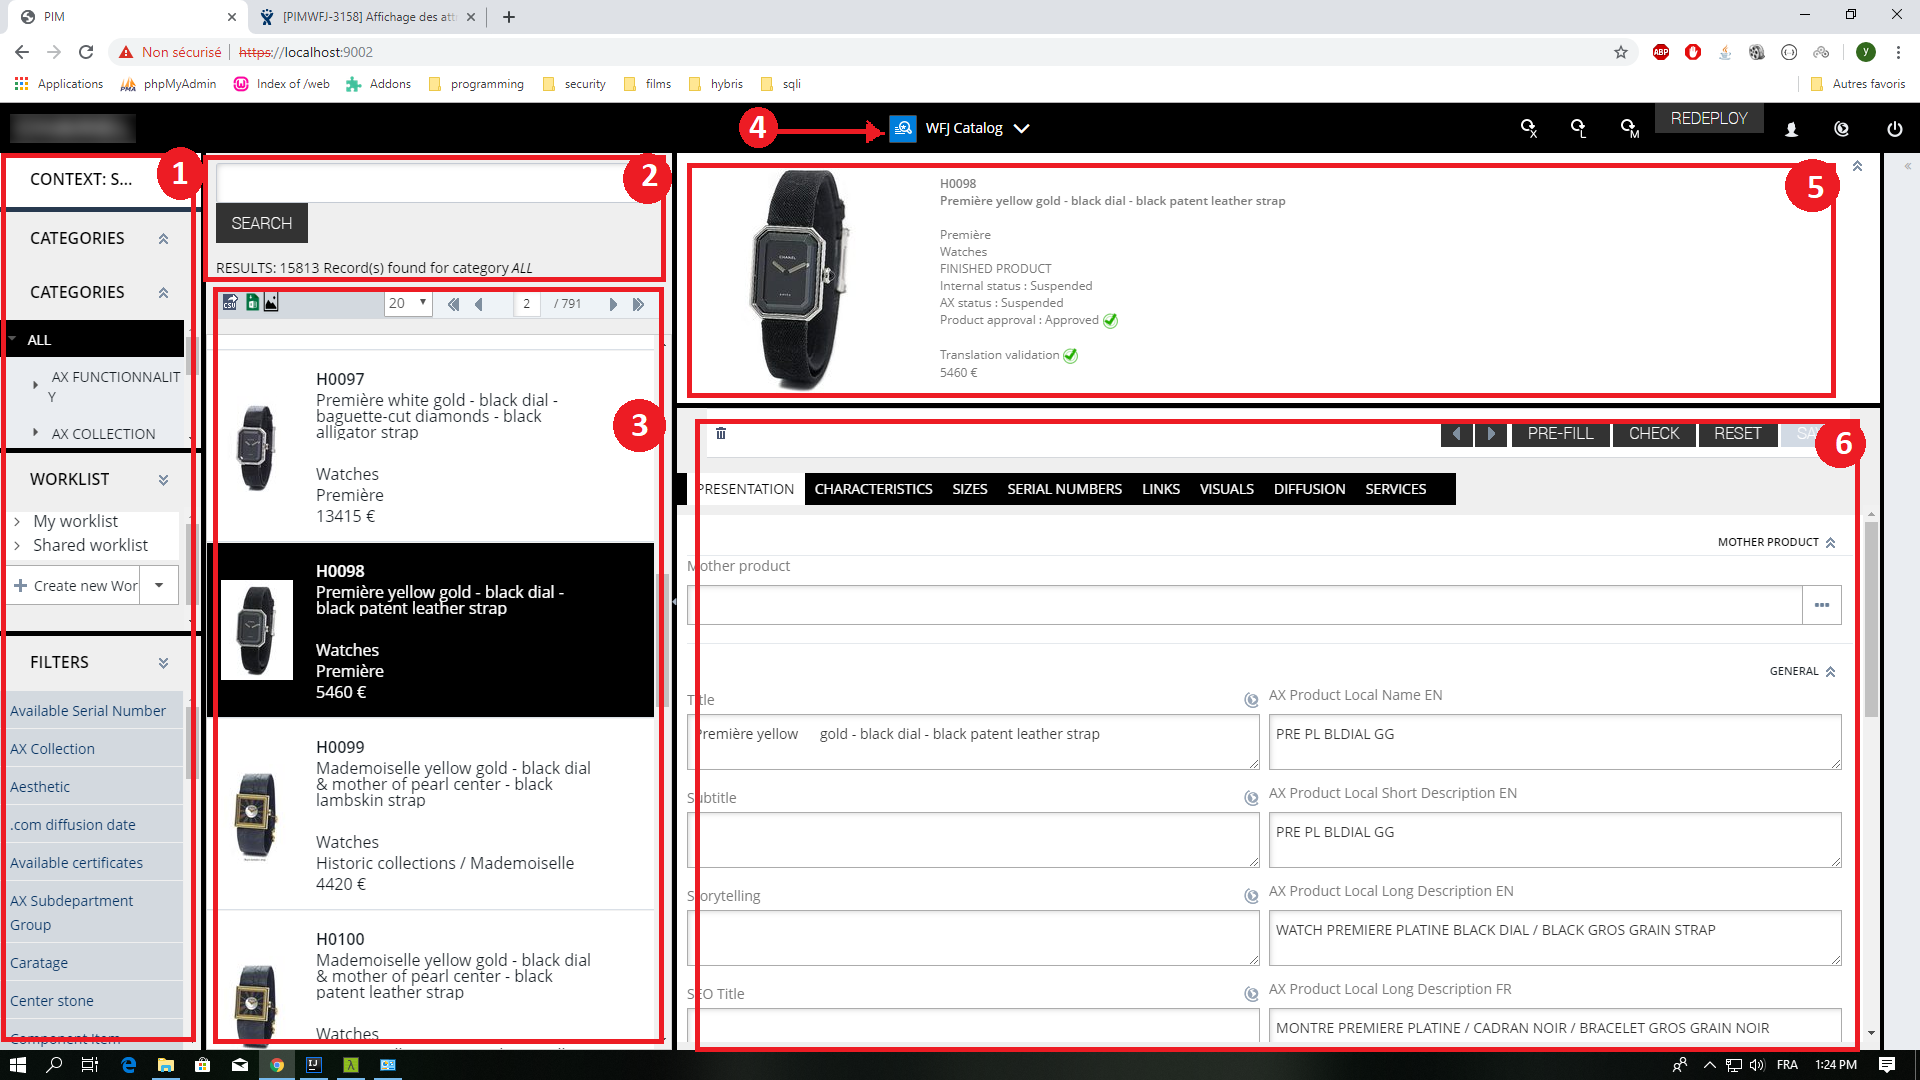
\includegraphics[width=16cm]{catalog_vue.PNG}
  \caption{La vue Catalogue de la plate-forme.}
  \label{fig:ctalog}
\end{figure}
\FloatBarrier

\subsection{La Vue Catégories}

La vue catégories La vue categories présenté dans la figure \ref{fig:category-vue} est une perspective qui permet de : 

\begin{itemize}
    \item[$\bullet$] Gérer les cétgories existantes au sein du PIM.
    \medskip
    \item[$\bullet$] Gérer des produits sur une catégorie sélectionnée, ie :
    \begin{itemize}
    \smallskip
        \item Rechercher des produits.
        \smallskip
        \item Associer des produits à une catégorie.
    \end{itemize}
\end{itemize}
\begin{figure}[ht]
  \centering
  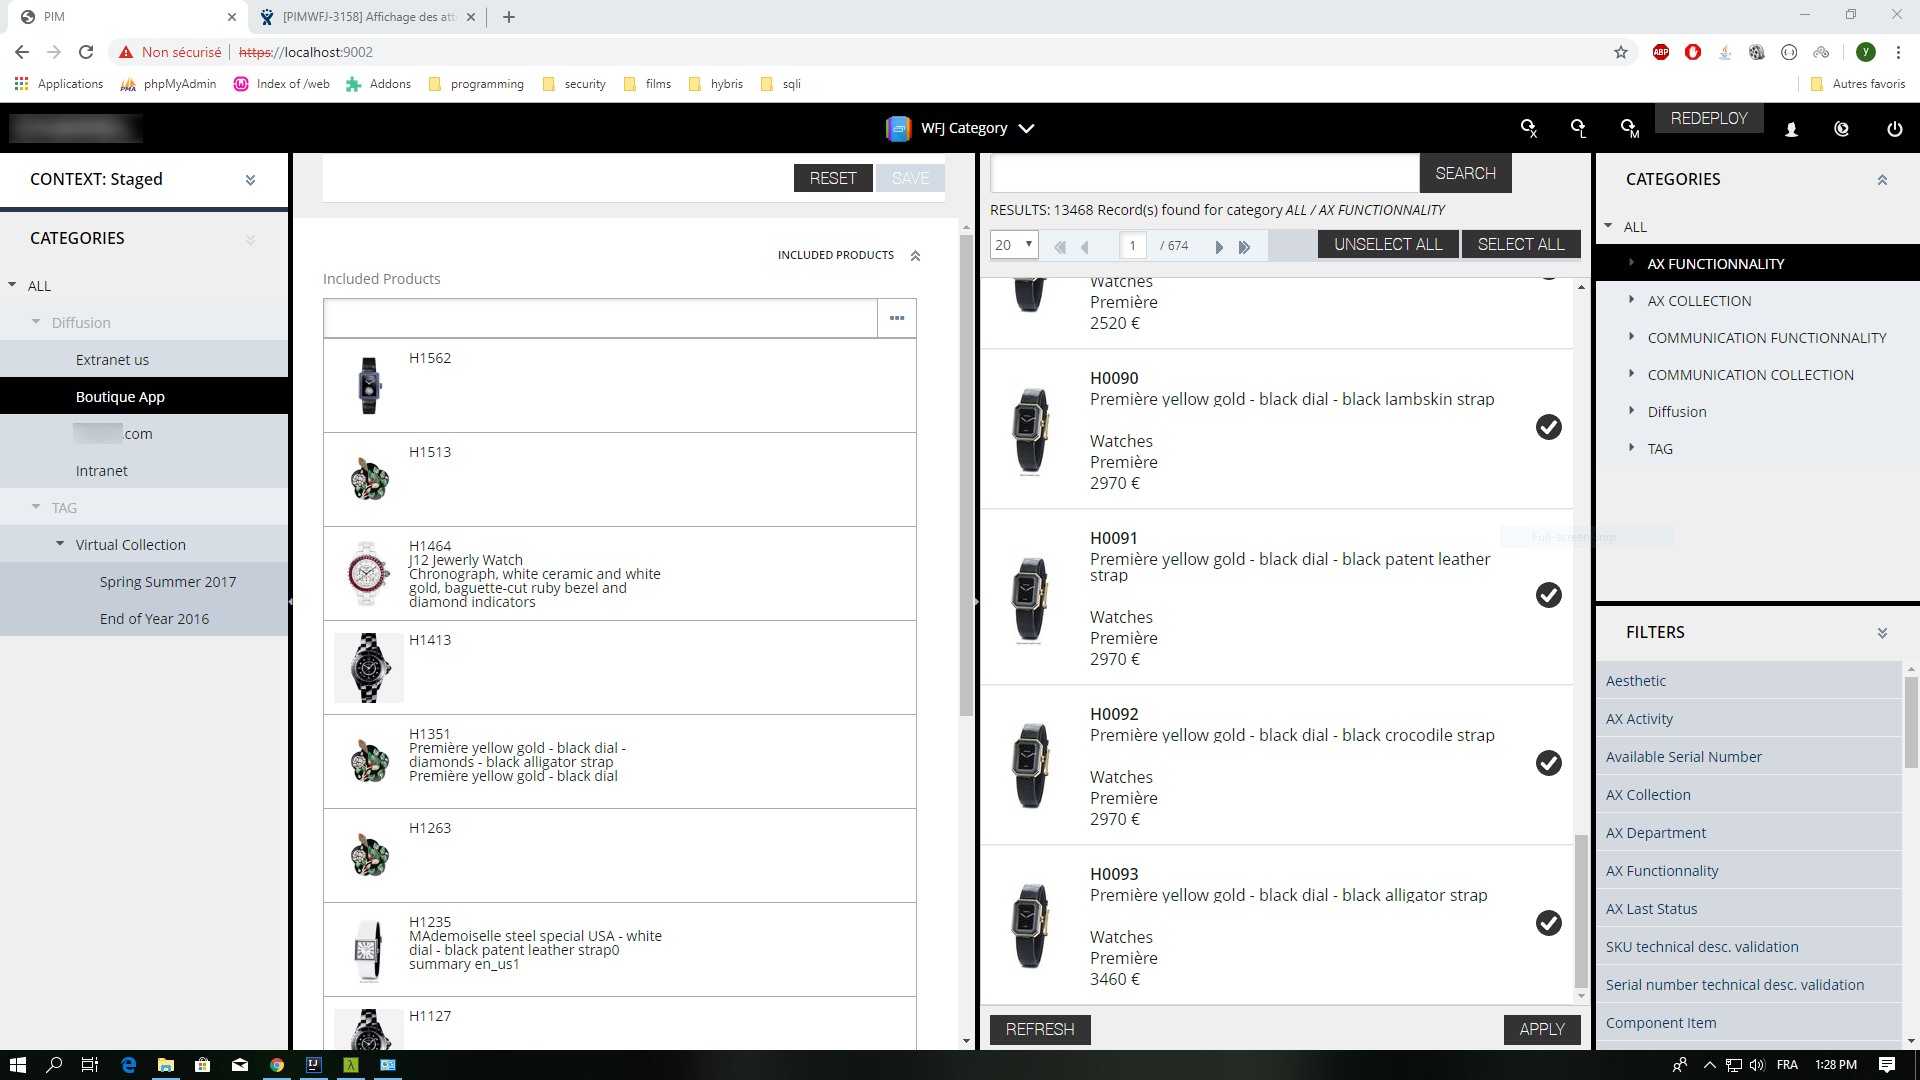
\includegraphics[width=16cm]{categories_vues.PNG}
  \caption{La vue Categories de la platforme.}
  \label{fig:category-vue}
\end{figure}
\FloatBarrier

\subsection{La Vue Dashboard}

Le dashboard WFJ permet d’afficher des indicateurs de suivi (voir la figure \ref{fig:dashboard}):

\begin{itemize}
    \item Un dashboard par statut (Approval Status) qui permet de voir le statut des produits par catégories (collection de communication).
    \smallskip
    \item Un dashboard qui indique le nombre de produits créés sur les 12 derniers mois.
    \smallskip
    \item Un dashboard pour les traductions par langue qui indique les produits qui ne sont pas traduits.
    
\end{itemize}

\begin{figure}[ht]
  \centering
  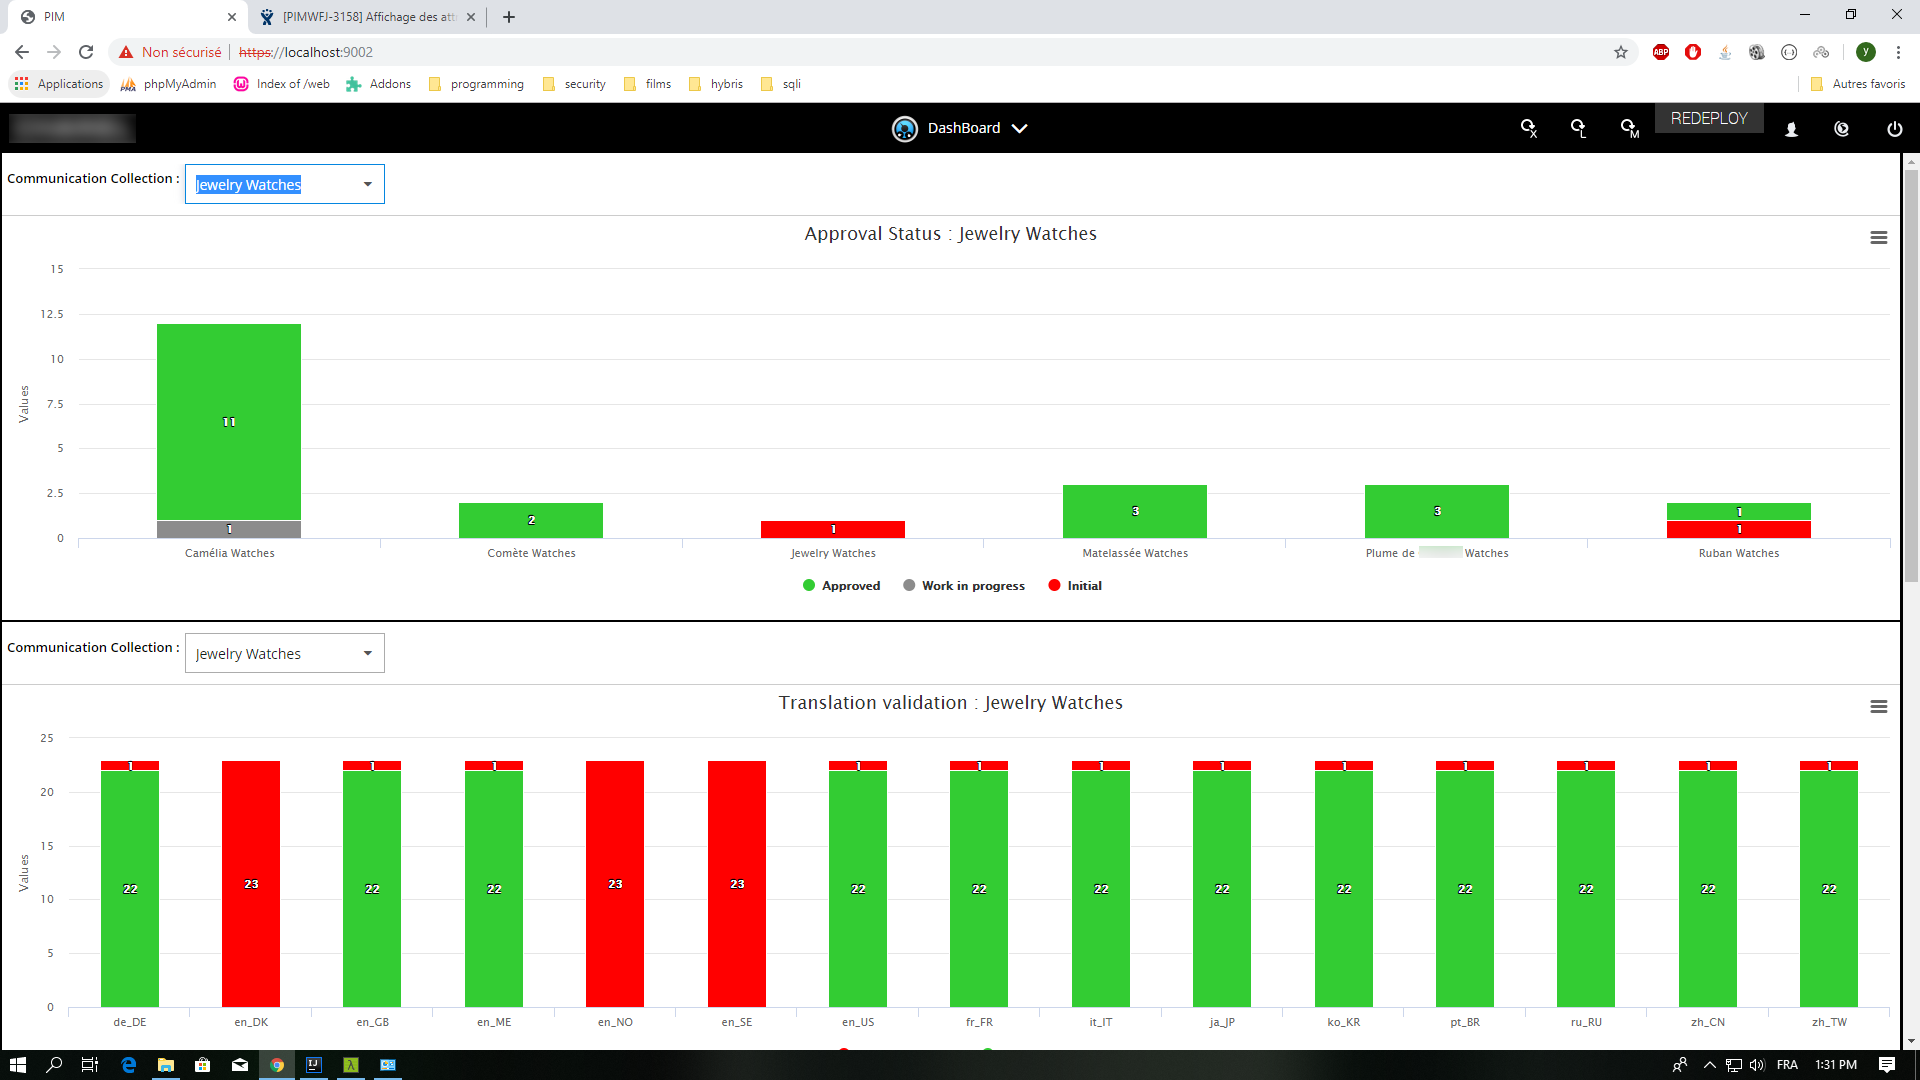
\includegraphics[width=16cm]{dashboard.PNG}
  \caption{La vue Dashboard de la plate-forme.}
  \label{fig:dashboard}
\end{figure}
\FloatBarrier

 


\section{Conclusion}
Dans ce chapitre, on a présenté la réalisation qu'on a effectué, l’environnement de développement, les outils et technologies utilisés dans le projet ainsi qu'une description détaillée des différentes interfaces utilisateur de la plate-forme.


